\documentclass{standalone}
\usepackage{tikz}
\usetikzlibrary{patterns, positioning}

\begin{document}
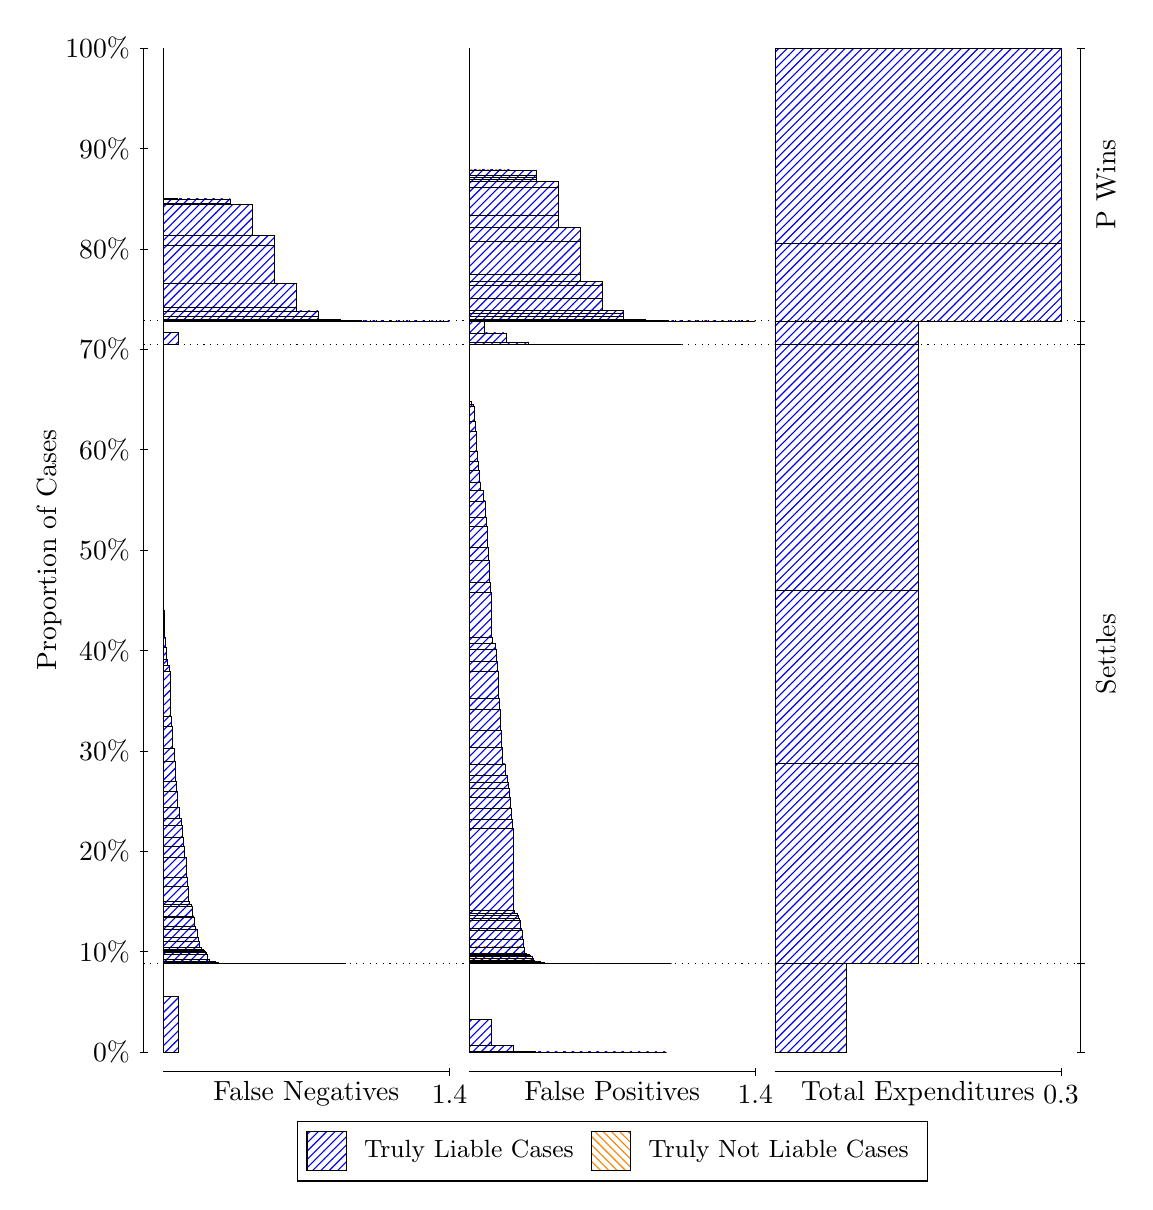
\begin{tikzpicture}
\draw[black, very thin] (1.5,1.75) -- (1.5,14.5);
\node[rotate=90, anchor=center] at (0.3, 8.125) {Proportion of Cases};
\draw[black, very thin] (1.45,1.75) -- (1.55,1.75);
\node[anchor=east] at (1.45, 1.75) {0\%};
\draw[black, very thin] (1.45,3.025) -- (1.55,3.025);
\node[anchor=east] at (1.45, 3.025) {10\%};
\draw[black, very thin] (1.45,4.3) -- (1.55,4.3);
\node[anchor=east] at (1.45, 4.3) {20\%};
\draw[black, very thin] (1.45,5.575) -- (1.55,5.575);
\node[anchor=east] at (1.45, 5.575) {30\%};
\draw[black, very thin] (1.45,6.85) -- (1.55,6.85);
\node[anchor=east] at (1.45, 6.85) {40\%};
\draw[black, very thin] (1.45,8.125) -- (1.55,8.125);
\node[anchor=east] at (1.45, 8.125) {50\%};
\draw[black, very thin] (1.45,9.4) -- (1.55,9.4);
\node[anchor=east] at (1.45, 9.4) {60\%};
\draw[black, very thin] (1.45,10.675) -- (1.55,10.675);
\node[anchor=east] at (1.45, 10.675) {70\%};
\draw[black, very thin] (1.45,11.95) -- (1.55,11.95);
\node[anchor=east] at (1.45, 11.95) {80\%};
\draw[black, very thin] (1.45,13.225) -- (1.55,13.225);
\node[anchor=east] at (1.45, 13.225) {90\%};
\draw[black, very thin] (1.45,14.5) -- (1.55,14.5);
\node[anchor=east] at (1.45, 14.5) {100\%};

\draw[black, very thin] (13.4,1.75) -- (13.4,14.5);
\draw[black, very thin] (13.35,1.75) -- (13.45,1.75);
\node[anchor=west] at (13.35, 1.75) {};
\draw[black, very thin] (13.35,2.8721) -- (13.45,2.8721);
\node[anchor=west] at (13.35, 2.8721) {};
\draw[black, very thin] (13.35,10.734) -- (13.45,10.734);
\node[anchor=west] at (13.35, 10.734) {};
\draw[black, very thin] (13.35,11.036) -- (13.45,11.036);
\node[anchor=west] at (13.35, 11.036) {};
\draw[black, very thin] (13.35,14.5) -- (13.45,14.5);
\node[anchor=west] at (13.35, 14.5) {};

\draw[black, very thin, pattern color=blue, pattern=north east lines] (1.75,1.75) rectangle (1.9379,2.4561);
\draw[black, very thin, pattern color=orange, pattern=north west lines] (1.75,2.4561) rectangle (1.75,2.4561);
\draw[black, very thin, pattern color=blue, pattern=north east lines] (1.75,2.4561) rectangle (1.75,2.8721);
\draw[black, very thin, pattern color=blue, pattern=north east lines] (1.75,2.8721) rectangle (4.0678,2.8721);
\draw[black, very thin, pattern color=blue, pattern=north east lines] (1.75,2.8721) rectangle (3.9425,2.8721);
\draw[black, very thin, pattern color=blue, pattern=north east lines] (1.75,2.8721) rectangle (3.8172,2.8721);
\draw[black, very thin, pattern color=blue, pattern=north east lines] (1.75,2.8721) rectangle (3.7894,2.8721);
\draw[black, very thin, pattern color=blue, pattern=north east lines] (1.75,2.8721) rectangle (3.692,2.8721);
\draw[black, very thin, pattern color=blue, pattern=north east lines] (1.75,2.8721) rectangle (3.6641,2.8721);
\draw[black, very thin, pattern color=blue, pattern=north east lines] (1.75,2.8721) rectangle (3.5667,2.8721);
\draw[black, very thin, pattern color=blue, pattern=north east lines] (1.75,2.8721) rectangle (3.5388,2.8721);
\draw[black, very thin, pattern color=blue, pattern=north east lines] (1.75,2.8721) rectangle (3.511,2.8721);
\draw[black, very thin, pattern color=blue, pattern=north east lines] (1.75,2.8721) rectangle (3.4414,2.8721);
\draw[black, very thin, pattern color=blue, pattern=north east lines] (1.75,2.8721) rectangle (3.4135,2.8721);
\draw[black, very thin, pattern color=blue, pattern=north east lines] (1.75,2.8721) rectangle (3.3857,2.8721);
\draw[black, very thin, pattern color=blue, pattern=north east lines] (1.75,2.8721) rectangle (3.3161,2.8721);
\draw[black, very thin, pattern color=blue, pattern=north east lines] (1.75,2.8721) rectangle (3.2883,2.8721);
\draw[black, very thin, pattern color=blue, pattern=north east lines] (1.75,2.8721) rectangle (3.2604,2.8721);
\draw[black, very thin, pattern color=blue, pattern=north east lines] (1.75,2.8721) rectangle (3.2326,2.8721);
\draw[black, very thin, pattern color=blue, pattern=north east lines] (1.75,2.8721) rectangle (3.1908,2.8721);
\draw[black, very thin, pattern color=blue, pattern=north east lines] (1.75,2.8721) rectangle (3.163,2.8721);
\draw[black, very thin, pattern color=blue, pattern=north east lines] (1.75,2.8721) rectangle (3.1351,2.8721);
\draw[black, very thin, pattern color=blue, pattern=north east lines] (1.75,2.8721) rectangle (3.1073,2.8721);
\draw[black, very thin, pattern color=blue, pattern=north east lines] (1.75,2.8721) rectangle (3.0655,2.8721);
\draw[black, very thin, pattern color=blue, pattern=north east lines] (1.75,2.8721) rectangle (3.0377,2.8721);
\draw[black, very thin, pattern color=blue, pattern=north east lines] (1.75,2.8721) rectangle (3.0098,2.8721);
\draw[black, very thin, pattern color=blue, pattern=north east lines] (1.75,2.8721) rectangle (2.982,2.8721);
\draw[black, very thin, pattern color=blue, pattern=north east lines] (1.75,2.8721) rectangle (2.9542,2.8721);
\draw[black, very thin, pattern color=blue, pattern=north east lines] (1.75,2.8721) rectangle (2.9402,2.8721);
\draw[black, very thin, pattern color=blue, pattern=north east lines] (1.75,2.8721) rectangle (2.9124,2.8721);
\draw[black, very thin, pattern color=blue, pattern=north east lines] (1.75,2.8721) rectangle (2.8845,2.8721);
\draw[black, very thin, pattern color=blue, pattern=north east lines] (1.75,2.8721) rectangle (2.8567,2.8721);
\draw[black, very thin, pattern color=blue, pattern=north east lines] (1.75,2.8721) rectangle (2.8289,2.8721);
\draw[black, very thin, pattern color=blue, pattern=north east lines] (1.75,2.8721) rectangle (2.8149,2.8721);
\draw[black, very thin, pattern color=blue, pattern=north east lines] (1.75,2.8721) rectangle (2.8149,2.8721);
\draw[black, very thin, pattern color=blue, pattern=north east lines] (1.75,2.8721) rectangle (2.7871,2.8721);
\draw[black, very thin, pattern color=blue, pattern=north east lines] (1.75,2.8721) rectangle (2.7593,2.8721);
\draw[black, very thin, pattern color=blue, pattern=north east lines] (1.75,2.8721) rectangle (2.7314,2.8722);
\draw[black, very thin, pattern color=blue, pattern=north east lines] (1.75,2.8722) rectangle (2.7036,2.8723);
\draw[black, very thin, pattern color=blue, pattern=north east lines] (1.75,2.8723) rectangle (2.6897,2.8723);
\draw[black, very thin, pattern color=blue, pattern=north east lines] (1.75,2.8723) rectangle (2.6757,2.8723);
\draw[black, very thin, pattern color=blue, pattern=north east lines] (1.75,2.8723) rectangle (2.6618,2.8723);
\draw[black, very thin, pattern color=blue, pattern=north east lines] (1.75,2.8723) rectangle (2.634,2.8724);
\draw[black, very thin, pattern color=blue, pattern=north east lines] (1.75,2.8724) rectangle (2.6061,2.8728);
\draw[black, very thin, pattern color=blue, pattern=north east lines] (1.75,2.8728) rectangle (2.5783,2.8734);
\draw[black, very thin, pattern color=blue, pattern=north east lines] (1.75,2.8734) rectangle (2.5644,2.8735);
\draw[black, very thin, pattern color=blue, pattern=north east lines] (1.75,2.8735) rectangle (2.5504,2.874);
\draw[black, very thin, pattern color=blue, pattern=north east lines] (1.75,2.874) rectangle (2.5365,2.874);
\draw[black, very thin, pattern color=blue, pattern=north east lines] (1.75,2.874) rectangle (2.5365,2.8742);
\draw[black, very thin, pattern color=blue, pattern=north east lines] (1.75,2.8742) rectangle (2.5087,2.8748);
\draw[black, very thin, pattern color=blue, pattern=north east lines] (1.75,2.8748) rectangle (2.4808,2.8795);
\draw[black, very thin, pattern color=blue, pattern=north east lines] (1.75,2.8795) rectangle (2.453,2.886);
\draw[black, very thin, pattern color=blue, pattern=north east lines] (1.75,2.886) rectangle (2.4391,2.8888);
\draw[black, very thin, pattern color=blue, pattern=north east lines] (1.75,2.8888) rectangle (2.4252,2.8954);
\draw[black, very thin, pattern color=blue, pattern=north east lines] (1.75,2.8954) rectangle (2.4112,2.896);
\draw[black, very thin, pattern color=blue, pattern=north east lines] (1.75,2.896) rectangle (2.3973,2.9016);
\draw[black, very thin, pattern color=blue, pattern=north east lines] (1.75,2.9016) rectangle (2.3834,2.9037);
\draw[black, very thin, pattern color=blue, pattern=north east lines] (1.75,2.9037) rectangle (2.3556,2.9056);
\draw[black, very thin, pattern color=blue, pattern=north east lines] (1.75,2.9056) rectangle (2.3277,2.9244);
\draw[black, very thin, pattern color=blue, pattern=north east lines] (1.75,2.9244) rectangle (2.3138,2.9944);
\draw[black, very thin, pattern color=blue, pattern=north east lines] (1.75,2.9944) rectangle (2.2999,3.0161);
\draw[black, very thin, pattern color=blue, pattern=north east lines] (1.75,3.0161) rectangle (2.286,3.0251);
\draw[black, very thin, pattern color=blue, pattern=north east lines] (1.75,3.0251) rectangle (2.272,3.0456);
\draw[black, very thin, pattern color=blue, pattern=north east lines] (1.75,3.0456) rectangle (2.2581,3.0457);
\draw[black, very thin, pattern color=blue, pattern=north east lines] (1.75,3.0457) rectangle (2.2581,3.0542);
\draw[black, very thin, pattern color=blue, pattern=north east lines] (1.75,3.0542) rectangle (2.2303,3.0759);
\draw[black, very thin, pattern color=blue, pattern=north east lines] (1.75,3.0759) rectangle (2.2024,3.1534);
\draw[black, very thin, pattern color=blue, pattern=north east lines] (1.75,3.1534) rectangle (2.1885,3.208);
\draw[black, very thin, pattern color=blue, pattern=north east lines] (1.75,3.208) rectangle (2.1746,3.3121);
\draw[black, very thin, pattern color=blue, pattern=north east lines] (1.75,3.3121) rectangle (2.1607,3.3504);
\draw[black, very thin, pattern color=blue, pattern=north east lines] (1.75,3.3504) rectangle (2.1467,3.4575);
\draw[black, very thin, pattern color=blue, pattern=north east lines] (1.75,3.4575) rectangle (2.1328,3.4774);
\draw[black, very thin, pattern color=blue, pattern=north east lines] (1.75,3.4774) rectangle (2.1189,3.5954);
\draw[black, very thin, pattern color=blue, pattern=north east lines] (1.75,3.5954) rectangle (2.105,3.6271);
\draw[black, very thin, pattern color=blue, pattern=north east lines] (1.75,3.6271) rectangle (2.0771,3.6585);
\draw[black, very thin, pattern color=blue, pattern=north east lines] (1.75,3.6585) rectangle (2.0632,3.8502);
\draw[black, very thin, pattern color=blue, pattern=north east lines] (1.75,3.8502) rectangle (2.0493,3.9701);
\draw[black, very thin, pattern color=blue, pattern=north east lines] (1.75,3.9701) rectangle (2.0354,4.2217);
\draw[black, very thin, pattern color=blue, pattern=north east lines] (1.75,4.2217) rectangle (2.0215,4.3603);
\draw[black, very thin, pattern color=blue, pattern=north east lines] (1.75,4.3603) rectangle (2.0075,4.4741);
\draw[black, very thin, pattern color=blue, pattern=north east lines] (1.75,4.4741) rectangle (1.9936,4.6235);
\draw[black, very thin, pattern color=blue, pattern=north east lines] (1.75,4.6235) rectangle (1.9797,4.6238);
\draw[black, very thin, pattern color=blue, pattern=north east lines] (1.75,4.6238) rectangle (1.9797,4.7191);
\draw[black, very thin, pattern color=blue, pattern=north east lines] (1.75,4.7191) rectangle (1.9519,4.8563);
\draw[black, very thin, pattern color=blue, pattern=north east lines] (1.75,4.8563) rectangle (1.924,5.0624);
\draw[black, very thin, pattern color=blue, pattern=north east lines] (1.75,5.0624) rectangle (1.9101,5.1831);
\draw[black, very thin, pattern color=blue, pattern=north east lines] (1.75,5.1831) rectangle (1.8962,5.4447);
\draw[black, very thin, pattern color=blue, pattern=north east lines] (1.75,5.4447) rectangle (1.8822,5.6082);
\draw[black, very thin, pattern color=blue, pattern=north east lines] (1.75,5.6082) rectangle (1.8683,5.8918);
\draw[black, very thin, pattern color=blue, pattern=north east lines] (1.75,5.8918) rectangle (1.8544,6.0125);
\draw[black, very thin, pattern color=blue, pattern=north east lines] (1.75,6.0125) rectangle (1.8405,6.5838);
\draw[black, very thin, pattern color=blue, pattern=north east lines] (1.75,6.5838) rectangle (1.8266,6.6632);
\draw[black, very thin, pattern color=blue, pattern=north east lines] (1.75,6.6632) rectangle (1.7987,6.7424);
\draw[black, very thin, pattern color=blue, pattern=north east lines] (1.75,6.7424) rectangle (1.7848,6.8924);
\draw[black, very thin, pattern color=blue, pattern=north east lines] (1.75,6.8924) rectangle (1.7709,7.0157);
\draw[black, very thin, pattern color=blue, pattern=north east lines] (1.75,7.0157) rectangle (1.757,7.3577);
\draw[black, very thin, pattern color=orange, pattern=north west lines] (1.75,7.3577) rectangle (1.75,7.3577);
\draw[black, very thin, pattern color=blue, pattern=north east lines] (1.75,7.3577) rectangle (1.75,10.734);
\draw[black, very thin, pattern color=blue, pattern=north east lines] (1.75,10.734) rectangle (1.9379,10.886);
\draw[black, very thin, pattern color=orange, pattern=north west lines] (1.75,10.886) rectangle (1.75,10.886);
\draw[black, very thin, pattern color=blue, pattern=north east lines] (1.75,10.886) rectangle (1.75,11.036);
\draw[black, very thin, pattern color=blue, pattern=north east lines] (1.75,11.036) rectangle (5.3833,11.036);
\draw[black, very thin, pattern color=blue, pattern=north east lines] (1.75,11.036) rectangle (5.1049,11.036);
\draw[black, very thin, pattern color=blue, pattern=north east lines] (1.75,11.036) rectangle (4.8265,11.036);
\draw[black, very thin, pattern color=blue, pattern=north east lines] (1.75,11.036) rectangle (4.8265,11.036);
\draw[black, very thin, pattern color=blue, pattern=north east lines] (1.75,11.036) rectangle (4.5481,11.036);
\draw[black, very thin, pattern color=blue, pattern=north east lines] (1.75,11.036) rectangle (4.2697,11.038);
\draw[black, very thin, pattern color=blue, pattern=north east lines] (1.75,11.038) rectangle (3.9913,11.057);
\draw[black, very thin, pattern color=blue, pattern=north east lines] (1.75,11.057) rectangle (3.7128,11.096);
\draw[black, very thin, pattern color=blue, pattern=north east lines] (1.75,11.096) rectangle (3.7128,11.161);
\draw[black, very thin, pattern color=blue, pattern=north east lines] (1.75,11.161) rectangle (3.4344,11.212);
\draw[black, very thin, pattern color=blue, pattern=north east lines] (1.75,11.212) rectangle (3.4344,11.51);
\draw[black, very thin, pattern color=blue, pattern=north east lines] (1.75,11.51) rectangle (3.3231,11.51);
\draw[black, very thin, pattern color=blue, pattern=north east lines] (1.75,11.51) rectangle (3.156,11.999);
\draw[black, very thin, pattern color=blue, pattern=north east lines] (1.75,11.999) rectangle (3.156,12.122);
\draw[black, very thin, pattern color=blue, pattern=north east lines] (1.75,12.122) rectangle (3.0446,12.122);
\draw[black, very thin, pattern color=blue, pattern=north east lines] (1.75,12.122) rectangle (3.0446,12.122);
\draw[black, very thin, pattern color=blue, pattern=north east lines] (1.75,12.122) rectangle (2.8776,12.518);
\draw[black, very thin, pattern color=blue, pattern=north east lines] (1.75,12.518) rectangle (2.7662,12.518);
\draw[black, very thin, pattern color=blue, pattern=north east lines] (1.75,12.518) rectangle (2.5992,12.523);
\draw[black, very thin, pattern color=blue, pattern=north east lines] (1.75,12.523) rectangle (2.5992,12.576);
\draw[black, very thin, pattern color=blue, pattern=north east lines] (1.75,12.576) rectangle (2.5992,12.583);
\draw[black, very thin, pattern color=blue, pattern=north east lines] (1.75,12.583) rectangle (2.4878,12.583);
\draw[black, very thin, pattern color=blue, pattern=north east lines] (1.75,12.583) rectangle (2.4878,12.583);
\draw[black, very thin, pattern color=blue, pattern=north east lines] (1.75,12.583) rectangle (2.3208,12.583);
\draw[black, very thin, pattern color=blue, pattern=north east lines] (1.75,12.583) rectangle (2.3208,12.583);
\draw[black, very thin, pattern color=blue, pattern=north east lines] (1.75,12.583) rectangle (2.2094,12.583);
\draw[black, very thin, pattern color=blue, pattern=north east lines] (1.75,12.583) rectangle (2.2094,12.583);
\draw[black, very thin, pattern color=blue, pattern=north east lines] (1.75,12.583) rectangle (2.0423,12.583);
\draw[black, very thin, pattern color=blue, pattern=north east lines] (1.75,12.583) rectangle (2.0423,12.583);
\draw[black, very thin, pattern color=blue, pattern=north east lines] (1.75,12.583) rectangle (1.931,12.584);
\draw[black, very thin, pattern color=blue, pattern=north east lines] (1.75,12.584) rectangle (1.931,12.59);
\draw[black, very thin, pattern color=blue, pattern=north east lines] (1.75,12.59) rectangle (1.7639,12.59);
\draw[black, very thin, pattern color=blue, pattern=north east lines] (1.75,12.59) rectangle (1.7639,12.59);
\draw[black, very thin, pattern color=orange, pattern=north west lines] (1.75,12.59) rectangle (1.75,12.59);
\draw[black, very thin, pattern color=blue, pattern=north east lines] (1.75,12.59) rectangle (1.75,14.5);
\draw[black, very thin, pattern color=orange, pattern=north west lines] (5.6333,1.75) rectangle (8.1391,1.75);
\draw[black, very thin, pattern color=blue, pattern=north east lines] (5.6333,1.75) rectangle (8.1391,1.75);
\draw[black, very thin, pattern color=blue, pattern=north east lines] (5.6333,1.75) rectangle (7.8607,1.75);
\draw[black, very thin, pattern color=blue, pattern=north east lines] (5.6333,1.75) rectangle (7.5822,1.75);
\draw[black, very thin, pattern color=blue, pattern=north east lines] (5.6333,1.75) rectangle (7.3038,1.75);
\draw[black, very thin, pattern color=blue, pattern=north east lines] (5.6333,1.75) rectangle (7.0254,1.75);
\draw[black, very thin, pattern color=blue, pattern=north east lines] (5.6333,1.75) rectangle (6.747,1.7503);
\draw[black, very thin, pattern color=blue, pattern=north east lines] (5.6333,1.7503) rectangle (6.4686,1.7579);
\draw[black, very thin, pattern color=blue, pattern=north east lines] (5.6333,1.7579) rectangle (6.1902,1.8357);
\draw[black, very thin, pattern color=blue, pattern=north east lines] (5.6333,1.8357) rectangle (5.9117,2.166);
\draw[black, very thin, pattern color=blue, pattern=north east lines] (5.6333,2.166) rectangle (5.6333,2.8721);
\draw[black, very thin, pattern color=orange, pattern=north west lines] (5.6333,2.8721) rectangle (8.2017,2.8721);
\draw[black, very thin, pattern color=blue, pattern=north east lines] (5.6333,2.8721) rectangle (8.2017,2.8721);
\draw[black, very thin, pattern color=orange, pattern=north west lines] (5.6333,2.8721) rectangle (8.0764,2.8721);
\draw[black, very thin, pattern color=blue, pattern=north east lines] (5.6333,2.8721) rectangle (8.0764,2.8721);
\draw[black, very thin, pattern color=orange, pattern=north west lines] (5.6333,2.8721) rectangle (7.9511,2.8721);
\draw[black, very thin, pattern color=blue, pattern=north east lines] (5.6333,2.8721) rectangle (7.9511,2.8721);
\draw[black, very thin, pattern color=blue, pattern=north east lines] (5.6333,2.8721) rectangle (7.9233,2.8721);
\draw[black, very thin, pattern color=orange, pattern=north west lines] (5.6333,2.8721) rectangle (7.8259,2.8721);
\draw[black, very thin, pattern color=blue, pattern=north east lines] (5.6333,2.8721) rectangle (7.8259,2.8721);
\draw[black, very thin, pattern color=blue, pattern=north east lines] (5.6333,2.8721) rectangle (7.798,2.8721);
\draw[black, very thin, pattern color=orange, pattern=north west lines] (5.6333,2.8721) rectangle (7.7006,2.8721);
\draw[black, very thin, pattern color=blue, pattern=north east lines] (5.6333,2.8721) rectangle (7.7006,2.8721);
\draw[black, very thin, pattern color=blue, pattern=north east lines] (5.6333,2.8721) rectangle (7.6727,2.8721);
\draw[black, very thin, pattern color=blue, pattern=north east lines] (5.6333,2.8721) rectangle (7.6449,2.8721);
\draw[black, very thin, pattern color=orange, pattern=north west lines] (5.6333,2.8721) rectangle (7.5753,2.8721);
\draw[black, very thin, pattern color=blue, pattern=north east lines] (5.6333,2.8721) rectangle (7.5753,2.8721);
\draw[black, very thin, pattern color=blue, pattern=north east lines] (5.6333,2.8721) rectangle (7.5474,2.8721);
\draw[black, very thin, pattern color=blue, pattern=north east lines] (5.6333,2.8721) rectangle (7.5196,2.8721);
\draw[black, very thin, pattern color=orange, pattern=north west lines] (5.6333,2.8721) rectangle (7.45,2.8721);
\draw[black, very thin, pattern color=blue, pattern=north east lines] (5.6333,2.8721) rectangle (7.45,2.8721);
\draw[black, very thin, pattern color=orange, pattern=north west lines] (5.6333,2.8721) rectangle (7.45,2.8721);
\draw[black, very thin, pattern color=blue, pattern=north east lines] (5.6333,2.8721) rectangle (7.45,2.8721);
\draw[black, very thin, pattern color=blue, pattern=north east lines] (5.6333,2.8721) rectangle (7.4222,2.8721);
\draw[black, very thin, pattern color=blue, pattern=north east lines] (5.6333,2.8721) rectangle (7.3943,2.8721);
\draw[black, very thin, pattern color=blue, pattern=north east lines] (5.6333,2.8721) rectangle (7.3665,2.8721);
\draw[black, very thin, pattern color=orange, pattern=north west lines] (5.6333,2.8721) rectangle (7.3247,2.8721);
\draw[black, very thin, pattern color=blue, pattern=north east lines] (5.6333,2.8721) rectangle (7.3247,2.8721);
\draw[black, very thin, pattern color=blue, pattern=north east lines] (5.6333,2.8721) rectangle (7.2969,2.8721);
\draw[black, very thin, pattern color=blue, pattern=north east lines] (5.6333,2.8721) rectangle (7.269,2.8721);
\draw[black, very thin, pattern color=blue, pattern=north east lines] (5.6333,2.8721) rectangle (7.2412,2.8721);
\draw[black, very thin, pattern color=orange, pattern=north west lines] (5.6333,2.8721) rectangle (7.1994,2.8721);
\draw[black, very thin, pattern color=blue, pattern=north east lines] (5.6333,2.8721) rectangle (7.1994,2.8721);
\draw[black, very thin, pattern color=blue, pattern=north east lines] (5.6333,2.8721) rectangle (7.1716,2.8721);
\draw[black, very thin, pattern color=blue, pattern=north east lines] (5.6333,2.8721) rectangle (7.1716,2.8721);
\draw[black, very thin, pattern color=blue, pattern=north east lines] (5.6333,2.8721) rectangle (7.1437,2.8721);
\draw[black, very thin, pattern color=blue, pattern=north east lines] (5.6333,2.8721) rectangle (7.1159,2.8721);
\draw[black, very thin, pattern color=blue, pattern=north east lines] (5.6333,2.8721) rectangle (7.0881,2.8721);
\draw[black, very thin, pattern color=orange, pattern=north west lines] (5.6333,2.8721) rectangle (7.0741,2.8721);
\draw[black, very thin, pattern color=blue, pattern=north east lines] (5.6333,2.8721) rectangle (7.0741,2.8721);
\draw[black, very thin, pattern color=blue, pattern=north east lines] (5.6333,2.8721) rectangle (7.0463,2.8721);
\draw[black, very thin, pattern color=blue, pattern=north east lines] (5.6333,2.8721) rectangle (7.0185,2.8721);
\draw[black, very thin, pattern color=blue, pattern=north east lines] (5.6333,2.8721) rectangle (6.9906,2.8721);
\draw[black, very thin, pattern color=blue, pattern=north east lines] (5.6333,2.8721) rectangle (6.9628,2.8721);
\draw[black, very thin, pattern color=orange, pattern=north west lines] (5.6333,2.8721) rectangle (6.9489,2.8721);
\draw[black, very thin, pattern color=blue, pattern=north east lines] (5.6333,2.8721) rectangle (6.9489,2.8721);
\draw[black, very thin, pattern color=blue, pattern=north east lines] (5.6333,2.8721) rectangle (6.921,2.8721);
\draw[black, very thin, pattern color=blue, pattern=north east lines] (5.6333,2.8721) rectangle (6.8932,2.8721);
\draw[black, very thin, pattern color=blue, pattern=north east lines] (5.6333,2.8721) rectangle (6.8932,2.8721);
\draw[black, very thin, pattern color=blue, pattern=north east lines] (5.6333,2.8721) rectangle (6.8653,2.8722);
\draw[black, very thin, pattern color=blue, pattern=north east lines] (5.6333,2.8722) rectangle (6.8375,2.8722);
\draw[black, very thin, pattern color=orange, pattern=north west lines] (5.6333,2.8722) rectangle (6.8236,2.8722);
\draw[black, very thin, pattern color=blue, pattern=north east lines] (5.6333,2.8722) rectangle (6.8236,2.8723);
\draw[black, very thin, pattern color=blue, pattern=north east lines] (5.6333,2.8723) rectangle (6.8096,2.8723);
\draw[black, very thin, pattern color=blue, pattern=north east lines] (5.6333,2.8723) rectangle (6.7957,2.8723);
\draw[black, very thin, pattern color=blue, pattern=north east lines] (5.6333,2.8723) rectangle (6.7679,2.8723);
\draw[black, very thin, pattern color=blue, pattern=north east lines] (5.6333,2.8723) rectangle (6.74,2.8728);
\draw[black, very thin, pattern color=blue, pattern=north east lines] (5.6333,2.8728) rectangle (6.7122,2.8733);
\draw[black, very thin, pattern color=orange, pattern=north west lines] (5.6333,2.8733) rectangle (6.6983,2.8733);
\draw[black, very thin, pattern color=blue, pattern=north east lines] (5.6333,2.8733) rectangle (6.6983,2.8734);
\draw[black, very thin, pattern color=blue, pattern=north east lines] (5.6333,2.8734) rectangle (6.6844,2.8737);
\draw[black, very thin, pattern color=blue, pattern=north east lines] (5.6333,2.8737) rectangle (6.6704,2.8738);
\draw[black, very thin, pattern color=blue, pattern=north east lines] (5.6333,2.8738) rectangle (6.6426,2.8744);
\draw[black, very thin, pattern color=blue, pattern=north east lines] (5.6333,2.8744) rectangle (6.6148,2.8791);
\draw[black, very thin, pattern color=blue, pattern=north east lines] (5.6333,2.8791) rectangle (6.6148,2.8791);
\draw[black, very thin, pattern color=blue, pattern=north east lines] (5.6333,2.8791) rectangle (6.5869,2.8857);
\draw[black, very thin, pattern color=orange, pattern=north west lines] (5.6333,2.8857) rectangle (6.573,2.8857);
\draw[black, very thin, pattern color=blue, pattern=north east lines] (5.6333,2.8857) rectangle (6.573,2.887);
\draw[black, very thin, pattern color=blue, pattern=north east lines] (5.6333,2.887) rectangle (6.5591,2.8931);
\draw[black, very thin, pattern color=blue, pattern=north east lines] (5.6333,2.8931) rectangle (6.5451,2.8939);
\draw[black, very thin, pattern color=blue, pattern=north east lines] (5.6333,2.8939) rectangle (6.5312,2.8957);
\draw[black, very thin, pattern color=blue, pattern=north east lines] (5.6333,2.8957) rectangle (6.5173,2.8977);
\draw[black, very thin, pattern color=blue, pattern=north east lines] (5.6333,2.8977) rectangle (6.4895,2.8997);
\draw[black, very thin, pattern color=blue, pattern=north east lines] (5.6333,2.8997) rectangle (6.4616,2.9184);
\draw[black, very thin, pattern color=orange, pattern=north west lines] (5.6333,2.9184) rectangle (6.4477,2.9184);
\draw[black, very thin, pattern color=blue, pattern=north east lines] (5.6333,2.9184) rectangle (6.4477,2.9382);
\draw[black, very thin, pattern color=blue, pattern=north east lines] (5.6333,2.9382) rectangle (6.4338,2.9593);
\draw[black, very thin, pattern color=blue, pattern=north east lines] (5.6333,2.9593) rectangle (6.4199,2.9668);
\draw[black, very thin, pattern color=blue, pattern=north east lines] (5.6333,2.9668) rectangle (6.4059,2.9782);
\draw[black, very thin, pattern color=blue, pattern=north east lines] (5.6333,2.9782) rectangle (6.392,2.986);
\draw[black, very thin, pattern color=blue, pattern=north east lines] (5.6333,2.986) rectangle (6.3642,3.0076);
\draw[black, very thin, pattern color=blue, pattern=north east lines] (5.6333,3.0076) rectangle (6.3363,3.0851);
\draw[black, very thin, pattern color=blue, pattern=north east lines] (5.6333,3.0851) rectangle (6.3363,3.0851);
\draw[black, very thin, pattern color=orange, pattern=north west lines] (5.6333,3.0851) rectangle (6.3224,3.0851);
\draw[black, very thin, pattern color=blue, pattern=north east lines] (5.6333,3.0851) rectangle (6.3224,3.1861);
\draw[black, very thin, pattern color=blue, pattern=north east lines] (5.6333,3.1861) rectangle (6.3085,3.2915);
\draw[black, very thin, pattern color=blue, pattern=north east lines] (5.6333,3.2915) rectangle (6.2946,3.3184);
\draw[black, very thin, pattern color=blue, pattern=north east lines] (5.6333,3.3184) rectangle (6.2807,3.4255);
\draw[black, very thin, pattern color=blue, pattern=north east lines] (5.6333,3.4255) rectangle (6.2667,3.4468);
\draw[black, very thin, pattern color=blue, pattern=north east lines] (5.6333,3.4468) rectangle (6.2528,3.4835);
\draw[black, very thin, pattern color=blue, pattern=north east lines] (5.6333,3.4835) rectangle (6.2389,3.515);
\draw[black, very thin, pattern color=blue, pattern=north east lines] (5.6333,3.515) rectangle (6.211,3.5464);
\draw[black, very thin, pattern color=orange, pattern=north west lines] (5.6333,3.5464) rectangle (6.1971,3.5464);
\draw[black, very thin, pattern color=blue, pattern=north east lines] (5.6333,3.5464) rectangle (6.1971,4.5869);
\draw[black, very thin, pattern color=blue, pattern=north east lines] (5.6333,4.5869) rectangle (6.1832,4.706);
\draw[black, very thin, pattern color=blue, pattern=north east lines] (5.6333,4.706) rectangle (6.1693,4.847);
\draw[black, very thin, pattern color=blue, pattern=north east lines] (5.6333,4.847) rectangle (6.1554,4.9885);
\draw[black, very thin, pattern color=blue, pattern=north east lines] (5.6333,4.9885) rectangle (6.1414,5.0939);
\draw[black, very thin, pattern color=blue, pattern=north east lines] (5.6333,5.0939) rectangle (6.1275,5.1765);
\draw[black, very thin, pattern color=blue, pattern=north east lines] (5.6333,5.1765) rectangle (6.1136,5.2702);
\draw[black, very thin, pattern color=blue, pattern=north east lines] (5.6333,5.2702) rectangle (6.0858,5.4074);
\draw[black, very thin, pattern color=blue, pattern=north east lines] (5.6333,5.4074) rectangle (6.0579,5.6138);
\draw[black, very thin, pattern color=blue, pattern=north east lines] (5.6333,5.6138) rectangle (6.0579,5.614);
\draw[black, very thin, pattern color=blue, pattern=north east lines] (5.6333,5.614) rectangle (6.044,5.8351);
\draw[black, very thin, pattern color=blue, pattern=north east lines] (5.6333,5.8351) rectangle (6.0301,6.105);
\draw[black, very thin, pattern color=blue, pattern=north east lines] (5.6333,6.105) rectangle (6.0162,6.2481);
\draw[black, very thin, pattern color=blue, pattern=north east lines] (5.6333,6.2481) rectangle (6.0022,6.5901);
\draw[black, very thin, pattern color=blue, pattern=north east lines] (5.6333,6.5901) rectangle (5.9883,6.7134);
\draw[black, very thin, pattern color=blue, pattern=north east lines] (5.6333,6.7134) rectangle (5.9744,6.8634);
\draw[black, very thin, pattern color=blue, pattern=north east lines] (5.6333,6.8634) rectangle (5.9605,6.9426);
\draw[black, very thin, pattern color=blue, pattern=north east lines] (5.6333,6.9426) rectangle (5.9326,7.022);
\draw[black, very thin, pattern color=blue, pattern=north east lines] (5.6333,7.022) rectangle (5.9187,7.5933);
\draw[black, very thin, pattern color=blue, pattern=north east lines] (5.6333,7.5933) rectangle (5.9048,7.714);
\draw[black, very thin, pattern color=blue, pattern=north east lines] (5.6333,7.714) rectangle (5.8909,7.9976);
\draw[black, very thin, pattern color=blue, pattern=north east lines] (5.6333,7.9976) rectangle (5.8769,8.1611);
\draw[black, very thin, pattern color=blue, pattern=north east lines] (5.6333,8.1611) rectangle (5.863,8.4226);
\draw[black, very thin, pattern color=blue, pattern=north east lines] (5.6333,8.4226) rectangle (5.8491,8.5434);
\draw[black, very thin, pattern color=blue, pattern=north east lines] (5.6333,8.5434) rectangle (5.8352,8.7495);
\draw[black, very thin, pattern color=blue, pattern=north east lines] (5.6333,8.7495) rectangle (5.8073,8.8867);
\draw[black, very thin, pattern color=blue, pattern=north east lines] (5.6333,8.8867) rectangle (5.7795,8.982);
\draw[black, very thin, pattern color=blue, pattern=north east lines] (5.6333,8.982) rectangle (5.7795,8.9823);
\draw[black, very thin, pattern color=blue, pattern=north east lines] (5.6333,8.9823) rectangle (5.7656,9.1317);
\draw[black, very thin, pattern color=blue, pattern=north east lines] (5.6333,9.1317) rectangle (5.7517,9.2455);
\draw[black, very thin, pattern color=blue, pattern=north east lines] (5.6333,9.2455) rectangle (5.7377,9.3841);
\draw[black, very thin, pattern color=blue, pattern=north east lines] (5.6333,9.3841) rectangle (5.7238,9.6356);
\draw[black, very thin, pattern color=blue, pattern=north east lines] (5.6333,9.6356) rectangle (5.7099,9.7556);
\draw[black, very thin, pattern color=blue, pattern=north east lines] (5.6333,9.7556) rectangle (5.696,9.9473);
\draw[black, very thin, pattern color=blue, pattern=north east lines] (5.6333,9.9473) rectangle (5.6821,9.9787);
\draw[black, very thin, pattern color=blue, pattern=north east lines] (5.6333,9.9787) rectangle (5.6542,10.01);
\draw[black, very thin, pattern color=blue, pattern=north east lines] (5.6333,10.01) rectangle (5.6403,10.128);
\draw[black, very thin, pattern color=blue, pattern=north east lines] (5.6333,10.128) rectangle (5.6333,10.734);
\draw[black, very thin, pattern color=orange, pattern=north west lines] (5.6333,10.734) rectangle (8.327,10.734);
\draw[black, very thin, pattern color=blue, pattern=north east lines] (5.6333,10.734) rectangle (8.327,10.734);
\draw[black, very thin, pattern color=blue, pattern=north east lines] (5.6333,10.734) rectangle (8.0486,10.734);
\draw[black, very thin, pattern color=blue, pattern=north east lines] (5.6333,10.734) rectangle (7.7702,10.734);
\draw[black, very thin, pattern color=blue, pattern=north east lines] (5.6333,10.734) rectangle (7.4918,10.734);
\draw[black, very thin, pattern color=blue, pattern=north east lines] (5.6333,10.734) rectangle (7.2133,10.734);
\draw[black, very thin, pattern color=blue, pattern=north east lines] (5.6333,10.734) rectangle (6.9349,10.734);
\draw[black, very thin, pattern color=blue, pattern=north east lines] (5.6333,10.734) rectangle (6.6565,10.735);
\draw[black, very thin, pattern color=blue, pattern=north east lines] (5.6333,10.735) rectangle (6.3781,10.764);
\draw[black, very thin, pattern color=blue, pattern=north east lines] (5.6333,10.764) rectangle (6.0997,10.883);
\draw[black, very thin, pattern color=blue, pattern=north east lines] (5.6333,10.883) rectangle (5.8213,11.036);
\draw[black, very thin, pattern color=orange, pattern=north west lines] (5.6333,11.036) rectangle (9.2667,11.036);
\draw[black, very thin, pattern color=blue, pattern=north east lines] (5.6333,11.036) rectangle (9.2667,11.036);
\draw[black, very thin, pattern color=orange, pattern=north west lines] (5.6333,11.036) rectangle (8.9883,11.036);
\draw[black, very thin, pattern color=blue, pattern=north east lines] (5.6333,11.036) rectangle (8.9883,11.036);
\draw[black, very thin, pattern color=orange, pattern=north west lines] (5.6333,11.036) rectangle (8.7098,11.036);
\draw[black, very thin, pattern color=blue, pattern=north east lines] (5.6333,11.036) rectangle (8.7098,11.036);
\draw[black, very thin, pattern color=blue, pattern=north east lines] (5.6333,11.036) rectangle (8.7098,11.036);
\draw[black, very thin, pattern color=orange, pattern=north west lines] (5.6333,11.036) rectangle (8.4314,11.036);
\draw[black, very thin, pattern color=blue, pattern=north east lines] (5.6333,11.036) rectangle (8.4314,11.036);
\draw[black, very thin, pattern color=orange, pattern=north west lines] (5.6333,11.036) rectangle (8.153,11.036);
\draw[black, very thin, pattern color=blue, pattern=north east lines] (5.6333,11.036) rectangle (8.153,11.038);
\draw[black, very thin, pattern color=blue, pattern=north east lines] (5.6333,11.038) rectangle (7.8746,11.042);
\draw[black, very thin, pattern color=blue, pattern=north east lines] (5.6333,11.042) rectangle (7.8746,11.046);
\draw[black, very thin, pattern color=orange, pattern=north west lines] (5.6333,11.046) rectangle (7.8746,11.046);
\draw[black, very thin, pattern color=blue, pattern=north east lines] (5.6333,11.046) rectangle (7.8746,11.058);
\draw[black, very thin, pattern color=blue, pattern=north east lines] (5.6333,11.058) rectangle (7.5962,11.094);
\draw[black, very thin, pattern color=blue, pattern=north east lines] (5.6333,11.094) rectangle (7.5962,11.129);
\draw[black, very thin, pattern color=orange, pattern=north west lines] (5.6333,11.129) rectangle (7.5962,11.129);
\draw[black, very thin, pattern color=blue, pattern=north east lines] (5.6333,11.129) rectangle (7.5962,11.167);
\draw[black, very thin, pattern color=blue, pattern=north east lines] (5.6333,11.167) rectangle (7.3178,11.322);
\draw[black, very thin, pattern color=orange, pattern=north west lines] (5.6333,11.322) rectangle (7.3178,11.322);
\draw[black, very thin, pattern color=blue, pattern=north east lines] (5.6333,11.322) rectangle (7.3178,11.491);
\draw[black, very thin, pattern color=blue, pattern=north east lines] (5.6333,11.491) rectangle (7.3178,11.532);
\draw[black, very thin, pattern color=orange, pattern=north west lines] (5.6333,11.532) rectangle (7.2064,11.532);
\draw[black, very thin, pattern color=blue, pattern=north east lines] (5.6333,11.532) rectangle (7.2064,11.532);
\draw[black, very thin, pattern color=blue, pattern=north east lines] (5.6333,11.532) rectangle (7.0393,11.626);
\draw[black, very thin, pattern color=blue, pattern=north east lines] (5.6333,11.626) rectangle (7.0393,12.042);
\draw[black, very thin, pattern color=blue, pattern=north east lines] (5.6333,12.042) rectangle (7.0393,12.224);
\draw[black, very thin, pattern color=orange, pattern=north west lines] (5.6333,12.224) rectangle (6.928,12.224);
\draw[black, very thin, pattern color=blue, pattern=north east lines] (5.6333,12.224) rectangle (6.928,12.224);
\draw[black, very thin, pattern color=blue, pattern=north east lines] (5.6333,12.224) rectangle (6.7609,12.382);
\draw[black, very thin, pattern color=blue, pattern=north east lines] (5.6333,12.382) rectangle (6.7609,12.729);
\draw[black, very thin, pattern color=blue, pattern=north east lines] (5.6333,12.729) rectangle (6.7609,12.806);
\draw[black, very thin, pattern color=orange, pattern=north west lines] (5.6333,12.806) rectangle (6.6496,12.806);
\draw[black, very thin, pattern color=blue, pattern=north east lines] (5.6333,12.806) rectangle (6.6496,12.806);
\draw[black, very thin, pattern color=blue, pattern=north east lines] (5.6333,12.806) rectangle (6.6496,12.806);
\draw[black, very thin, pattern color=blue, pattern=north east lines] (5.6333,12.806) rectangle (6.4825,12.827);
\draw[black, very thin, pattern color=blue, pattern=north east lines] (5.6333,12.827) rectangle (6.4825,12.862);
\draw[black, very thin, pattern color=blue, pattern=north east lines] (5.6333,12.862) rectangle (6.4825,12.879);
\draw[black, very thin, pattern color=blue, pattern=north east lines] (5.6333,12.879) rectangle (6.4825,12.945);
\draw[black, very thin, pattern color=blue, pattern=north east lines] (5.6333,12.945) rectangle (6.3711,12.945);
\draw[black, very thin, pattern color=orange, pattern=north west lines] (5.6333,12.945) rectangle (6.3711,12.945);
\draw[black, very thin, pattern color=blue, pattern=north east lines] (5.6333,12.945) rectangle (6.3711,12.945);
\draw[black, very thin, pattern color=blue, pattern=north east lines] (5.6333,12.945) rectangle (6.2041,12.949);
\draw[black, very thin, pattern color=blue, pattern=north east lines] (5.6333,12.949) rectangle (6.2041,12.951);
\draw[black, very thin, pattern color=blue, pattern=north east lines] (5.6333,12.951) rectangle (6.2041,12.952);
\draw[black, very thin, pattern color=blue, pattern=north east lines] (5.6333,12.952) rectangle (6.0927,12.952);
\draw[black, very thin, pattern color=orange, pattern=north west lines] (5.6333,12.952) rectangle (6.0927,12.952);
\draw[black, very thin, pattern color=blue, pattern=north east lines] (5.6333,12.952) rectangle (6.0927,12.952);
\draw[black, very thin, pattern color=blue, pattern=north east lines] (5.6333,12.952) rectangle (6.0927,12.952);
\draw[black, very thin, pattern color=blue, pattern=north east lines] (5.6333,12.952) rectangle (5.9257,12.952);
\draw[black, very thin, pattern color=blue, pattern=north east lines] (5.6333,12.952) rectangle (5.9257,12.952);
\draw[black, very thin, pattern color=blue, pattern=north east lines] (5.6333,12.952) rectangle (5.8143,12.952);
\draw[black, very thin, pattern color=orange, pattern=north west lines] (5.6333,12.952) rectangle (5.8143,12.952);
\draw[black, very thin, pattern color=blue, pattern=north east lines] (5.6333,12.952) rectangle (5.8143,12.952);
\draw[black, very thin, pattern color=blue, pattern=north east lines] (5.6333,12.952) rectangle (5.8143,12.953);
\draw[black, very thin, pattern color=blue, pattern=north east lines] (5.6333,12.953) rectangle (5.6473,12.953);
\draw[black, very thin, pattern color=blue, pattern=north east lines] (5.6333,12.953) rectangle (5.6473,12.953);
\draw[black, very thin, pattern color=orange, pattern=north west lines] (5.6333,12.953) rectangle (5.6333,12.953);
\draw[black, very thin, pattern color=blue, pattern=north east lines] (5.6333,12.953) rectangle (5.6333,14.5);
\draw[black, very thin, pattern color=orange, pattern=north west lines] (9.5167,1.75) rectangle (10.425,1.75);
\draw[black, very thin, pattern color=blue, pattern=north east lines] (9.5167,1.75) rectangle (10.425,2.8721);
\draw[black, very thin, pattern color=orange, pattern=north west lines] (9.5167,2.8721) rectangle (11.333,2.8721);
\draw[black, very thin, pattern color=blue, pattern=north east lines] (9.5167,2.8721) rectangle (11.333,5.4146);
\draw[black, very thin, pattern color=orange, pattern=north west lines] (9.5167,5.4146) rectangle (11.333,5.4146);
\draw[black, very thin, pattern color=blue, pattern=north east lines] (9.5167,5.4146) rectangle (11.333,7.6151);
\draw[black, very thin, pattern color=orange, pattern=north west lines] (9.5167,7.6151) rectangle (11.333,7.6151);
\draw[black, very thin, pattern color=blue, pattern=north east lines] (9.5167,7.6151) rectangle (11.333,10.734);
\draw[black, very thin, pattern color=orange, pattern=north west lines] (9.5167,10.734) rectangle (11.333,10.734);
\draw[black, very thin, pattern color=blue, pattern=north east lines] (9.5167,10.734) rectangle (11.333,11.036);
\draw[black, very thin, pattern color=orange, pattern=north west lines] (9.5167,11.036) rectangle (13.15,11.036);
\draw[black, very thin, pattern color=blue, pattern=north east lines] (9.5167,11.036) rectangle (13.15,12.018);
\draw[black, very thin, pattern color=orange, pattern=north west lines] (9.5167,12.018) rectangle (13.15,12.018);
\draw[black, very thin, pattern color=blue, pattern=north east lines] (9.5167,12.018) rectangle (13.15,14.5);
\draw[black, dotted] (1.5,2.8721) -- (13.4,2.8721);
\draw[black, dotted] (1.5,10.734) -- (13.4,10.734);
\draw[black, dotted] (1.5,11.036) -- (13.4,11.036);
\draw[black, very thin] (1.75,1.5) -- (5.3833,1.5);
\node[anchor=north] at (3.5667, 1.5) {False Negatives};
\draw[black, very thin] (5.3833,1.45) -- (5.3833,1.55);
\node[anchor=north] at (5.3833, 1.45) {1.4};

\draw[black, very thin] (5.6333,1.5) -- (9.2667,1.5);
\node[anchor=north] at (7.45, 1.5) {False Positives};
\draw[black, very thin] (9.2667,1.45) -- (9.2667,1.55);
\node[anchor=north] at (9.2667, 1.45) {1.4};

\draw[black, very thin] (9.5167,1.5) -- (13.15,1.5);
\node[anchor=north] at (11.333, 1.5) {Total Expenditures};
\draw[black, very thin] (13.15,1.45) -- (13.15,1.55);
\node[anchor=north] at (13.15, 1.45) {0.3};


\node[black, centered, rotate=90] at (13.72, 6.8029) {Settles};

\node[black, centered, rotate=90] at (13.72, 12.768) {P Wins};

\draw (7.449999999999999,1.5) node[draw=none] (baseCoordinate) {};
\begin{scope}[align=center]
        \matrix[scale=0.5, draw=black, below=0.5cm of baseCoordinate, nodes={draw}, column sep=0.1cm]{
            \node[rectangle, draw, minimum width=0.5cm, minimum height=0.5cm, pattern=north east lines, pattern color=blue] {}; &
            \node[draw=none, font=\small] (B) {Truly Liable Cases}; &
            \node[rectangle, draw, minimum width=0.5cm, minimum height=0.5cm, pattern=north west lines, pattern color=orange] {}; &
            \node[draw=none, font=\small] (B) {Truly Not Liable Cases}; \\
            };
\end{scope}

\end{tikzpicture}
\end{document}